\documentclass{article}
\usepackage[top=1.00in, bottom=1.0in, left=1.00in, right=1.00in]{geometry}
\renewcommand{\baselinestretch}{1.1}
\usepackage{graphicx}
\usepackage{natbib}
\usepackage{amsmath}
\bibliographystyle{..//refs/styles/besjournals.bst}
\def\labelitemi{--}
\parindent=24pt
\usepackage{lineno}
\linenumbers
\usepackage{xr-hyper}
\externaldocument{write suppliment here}

\begin{document}
\section*{Introduction}

\section*{FLS hypotheses}
\begin{enumerate}
\item State hypotheses
\item Present available evidence, emphasize lack of synthesis.
\item Lack of a consensis stems from the fact that our current conceptual framework to describe FLS is disconnected from the underyling biology and the biological mechanisms we hope to test

\end{enumerate}

\section*{The current FLS framework and its limitations}
\begin{enumerate}
\item Ambiguous definitions
\item Categories may not be biologically meaningful, biased. Fig(2a)
\item Studies aknowledge there is likely high intraspecfic variation in FLS, yet FLS categories are applied at species level. If there is high intraspecific variation in it may alter or clarify the predictions of the hypotheses, yet it has never been systematically evaluated.
\item We evaluated intraspecific variation in two datasets and found it bit (fig 3,4)
\end{enumerate}
\section*{Intraspecific variation and the functional driver of FLS}
\section*{Future directions for the study of FLS}

\section*{Figures}
\begin{figure}[ht]
    \centering
 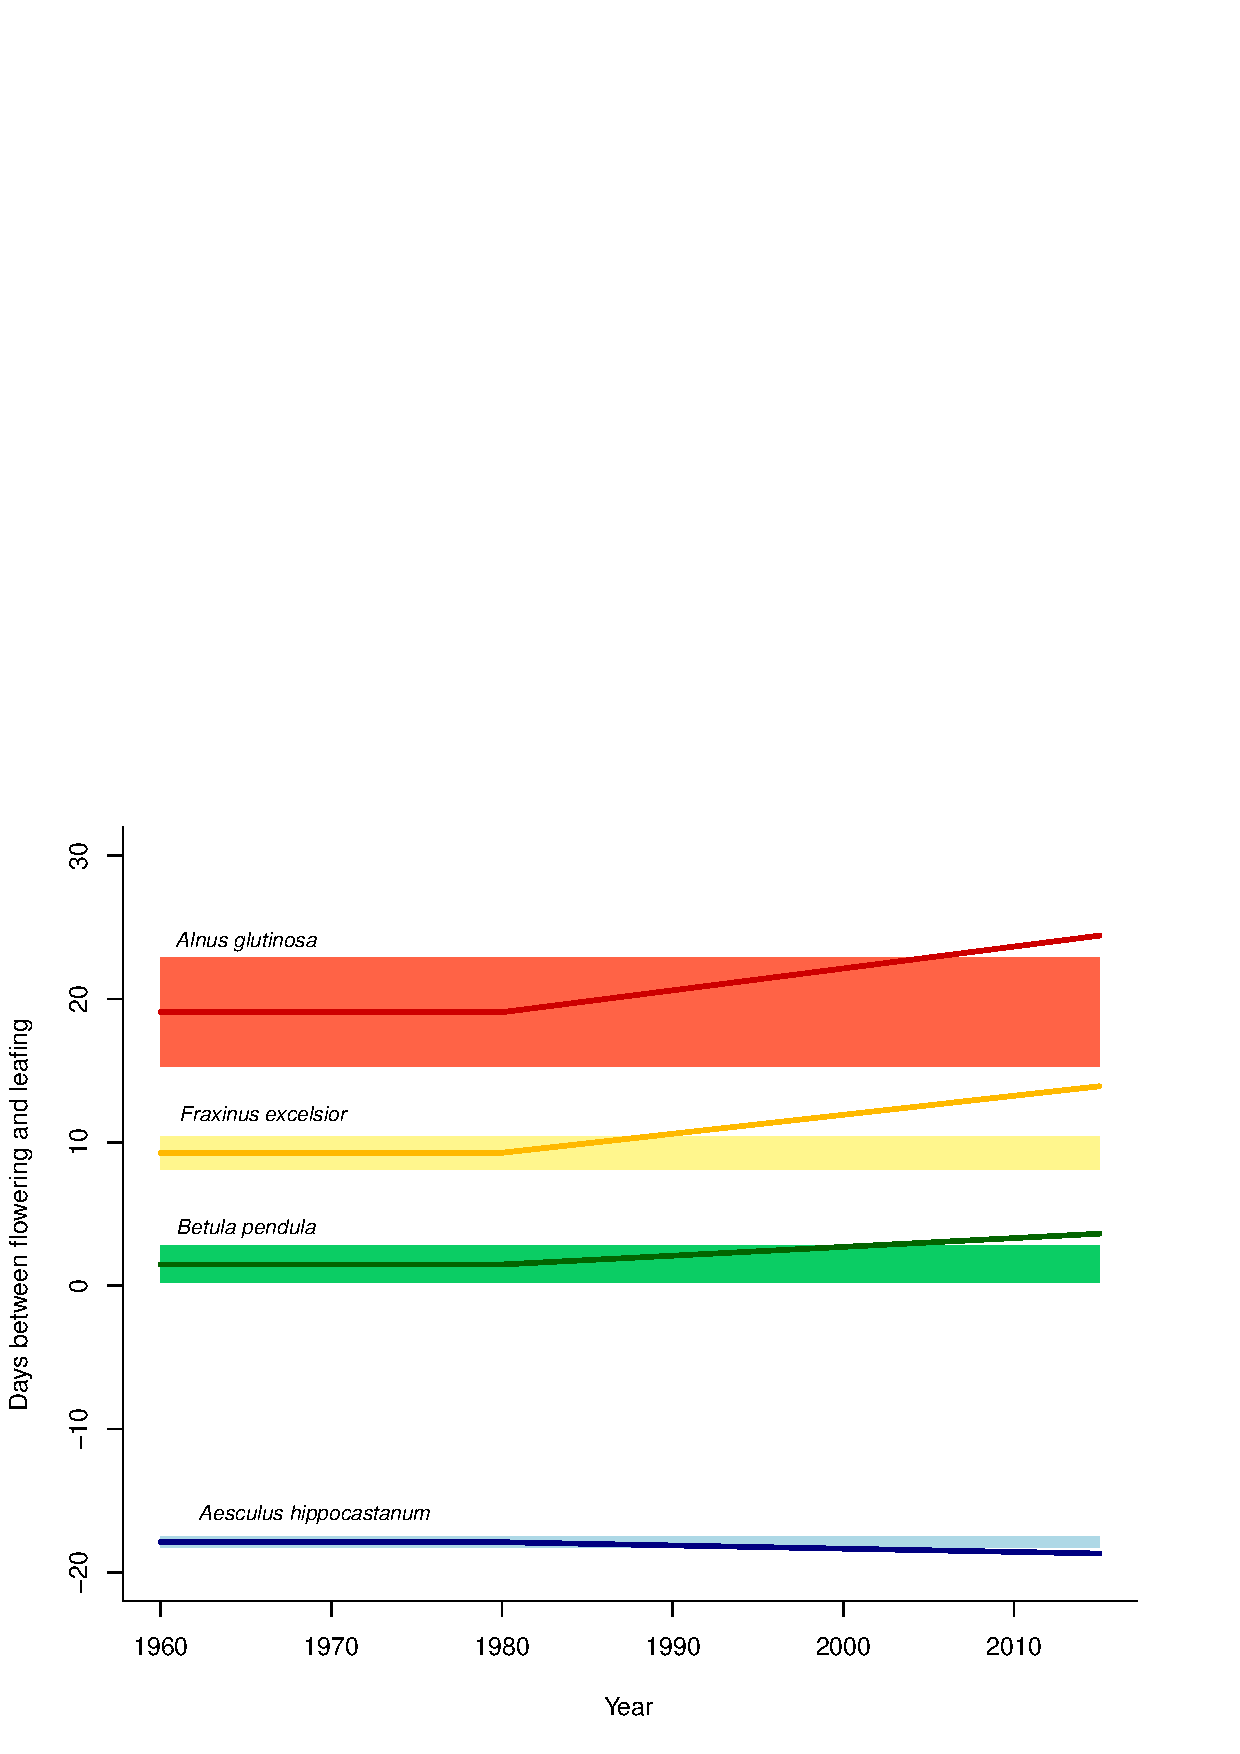
\includegraphics[width=\textwidth]{..//PEP725/FLS_climate_change.jpeg} 
    \caption{\textbf{FLSs across Europe for four tree species from 1960 to 2015 suggests climate change has generally increased the time between flowering and leafing}, but the direction and rate of change differs across species, which may exacerbate fitness differences within forest communities. To detect the effect of climate change on average FLS, we used models that allow for shifts in FLS after 1980. Lines represent the mean trend in FLS per species, and the highlighted regions indicate historic range of FLS variability (95\% credible intervals of the pre-1980 average) from the PEP725 database \citep{PEP725}.}
    \label{fig:climchange}
\end{figure}

  \begin{figure}[ht]
    \centering
    \includegraphics[width=\textwidth]{..//muplots.jpeg}
    \caption{\textbf{Estimated effects of water dynamics (minimum precipitation across species range), pollination syndrome, and earlier flowering time on FLS patterns across three case studies.} We used phylogenetic adjustments and standardized units to make a basic comparison of datasets of different  definitions of of FLS and  data types (categorical and continuous).  }
  \label{fig:muplots}
    \end{figure}

%\begin{figure}[ht]
 %   \centering
%    \includegraphics[width=\textwidth]{..//HarvardForest/HFmeans_expanded.jpeg}
 %   \caption{\textbf{Average inter-specific FLS variation at Harvard Forest, MA from 1990-2015.} This community displays all major FLS patterns, but because of overlapping floral and vegetative sub-phases and interannual variability in phenology (lines indicate standard error for each phenophase mean), it is difficult to neatly assign all species to a FLS category. Other notable patterns relevant to the FLS hypotheses can be seen. 1) As predicted by the early flowering hypothesis, the earliest species to initiate spring phenology are hysteranthous. 2) As predicted by the pollination syndrome hypothesis, wind-pollinated species (indicated with a *) may vary in whether their flowers or vegetative buds break first, but all open their flowers before leaves expand to 75\%.}
  %  \label{fig:HFmeans}
%\end{figure}

 \begin{figure}[ht]
        \centering
          \includegraphics[width=\textwidth]{..//HarvardForest/HF_Q_ru_interannual.jpeg}
          \caption{\textbf{Individual FLS variability over time for \textit{Quercus rubra} at Harvard Forest.} While this species is typically is classified as synanthous, we see here that the the order of flower and leaf bud break, and the time between these events varies considerably for each individual over time, and between individuals in any given year. None of this variation can be accounted for in a categorical FLS classification system.}
        \label{fig:Quercus}
    \end{figure}
    

 \begin{figure}[ht]
        \centering
          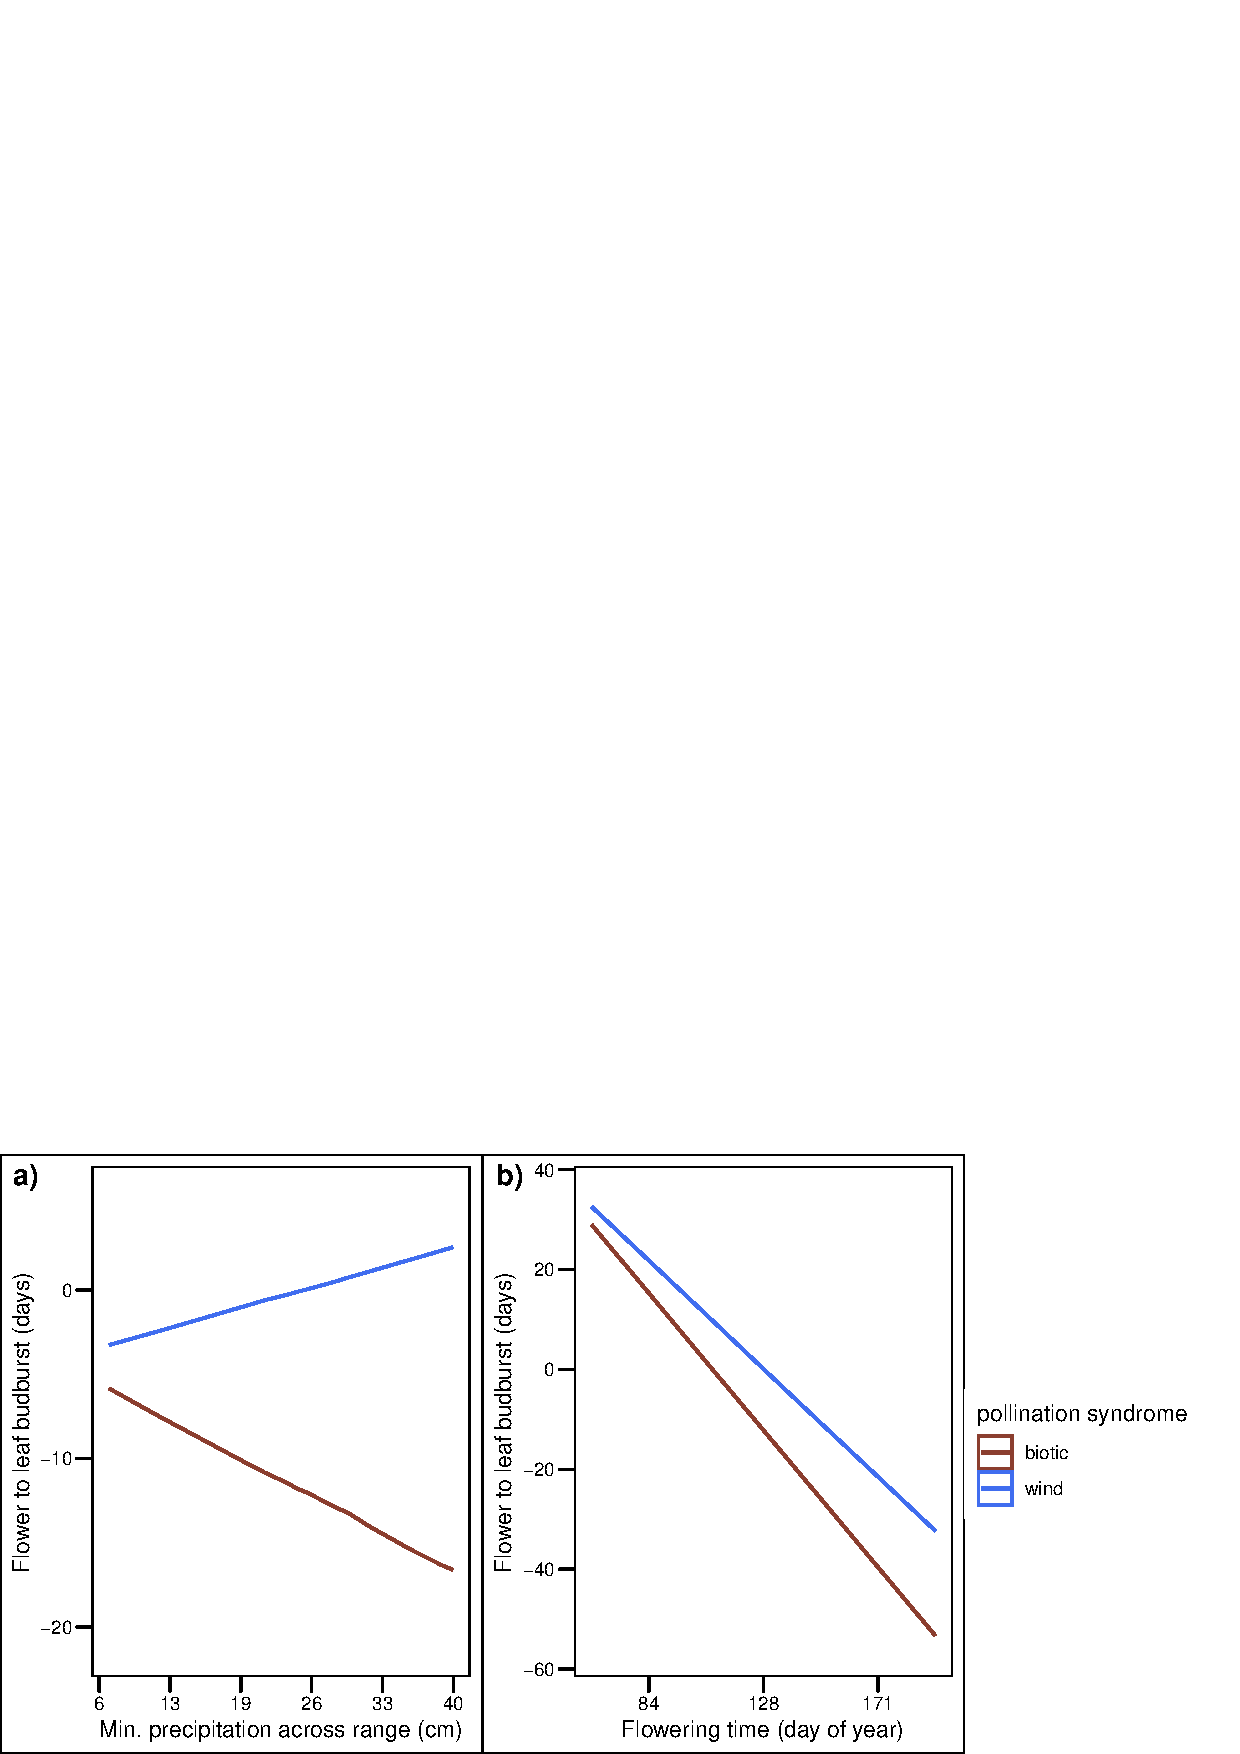
\includegraphics[width=\textwidth]{..//HarvardForest/apcs.jpeg}
           \caption{\textbf{Average predictive comparisons suggest that water dynamics may be a driver of hysteranthy in biotically-pollinated but not in wind-pollinated taxa, suggesting future work on FLS must accommodate overlapping hypotheses.} For species flowering in mid-May (the 25 year community average) these systematic differences}
        \label{fig:apcs}
    \end{figure}
\end{document}